%------------------------------------------------
\section{All Pairs Shortest Paths (APSP)} 

\subsection{Idee} 

\begin{frame}
\frametitle{APSP - All Pairs Shortest Paths}
\begin{block}{Problemstellung}
Man hat einen Graphen gegeben, der gewichtet ist. Nun möchte man den kürzesten Pfad zwischen allen Knoten i zu allen Knoten j herausfinden.
\end{block}
\end{frame}

%------------------------------------------------

\begin{frame}
\frametitle{APSP - Erster Ansatz}
\begin{block}{Lösungsansatz}
Man verwendet den bereits bekannten SSSP-Algorithmus, und führe diesen nach bedarf aus, d.h. in diesem Fall n-mal.
\end{block}

\begin{block}{Laufzeit}
$n \cdot O (m + n \cdot log(n))$\\$
= n \cdot O (n^2 + n \cdot log(n))$\\$ 
= n \cdot O (n^2 + n^2) $\\$ 
= O (n^3) $\\
$\implies$ geht es einfacher in etwa der selben Zeit?
\end{block}
\end{frame}

%------------------------------------------------

\begin{frame}
\frametitle{APSP - Zweiter Ansatz}
\begin{block}{Lösungsansatz}
Wir wissen: jeder Pfad zwischen zwei Knoten ist entweder bereits der kürzeste, oder es gibt einen Kürzeren Pfad als zwei Verknüpfung anderer Pfade über mindestens einen dritten Knoten.
\end{block}

\begin{block}{Genauer}
Systematisch in einer Adjazenzmatrix A:
Nehme für jeden Pfad $A[i][j] = \min\left(A[i][j], A[i][k] + A[i][k]\right)$, d.h. entweder der Pfad ist bereits minimal, oder ein Pfad über Knoten k ist kürzer und wird als neues Minimum übernommen.
Wenn man nun richtig iteriert, erhält man alle minimalen Pfade.
\end{block}
\end{frame}

%------------------------------------------------

\subsection{Code}

\begin{frame}[fragile] % Need to use the fragile option when verbatim is used in the slide
\frametitle{Code}

\begin{lstlisting}
for (int k = 0; k < V; k++)
    for (int i = 0; i < V; i++)
        for (int j = 0; j < V; j++)
            A[i][j] = min(
              A[i][j],
              A[i][k] + A[k][j]
            );
\end{lstlisting}

~\\$\implies$ der Aufwand liegt in $O(n^3)$

\end{frame}

%------------------------------------------------

\begin{frame}
\frametitle{Beispiel - Urzustand}

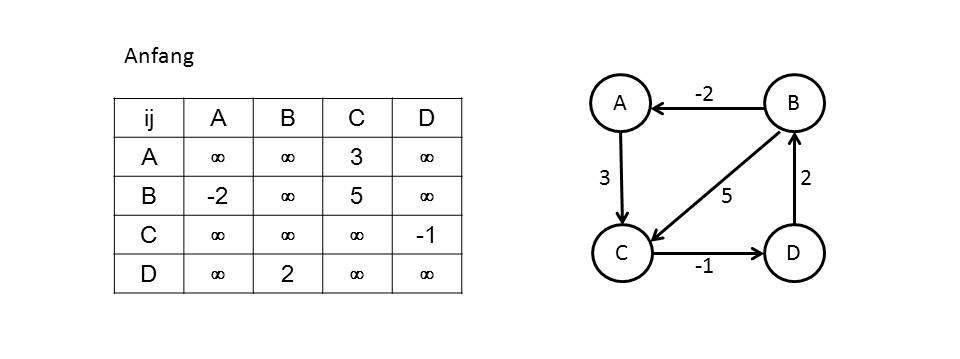
\includegraphics[width=\linewidth]{floyd_warshall_graphs/graph1.JPG}

\end{frame}

%------------------------------------------------

\begin{frame}
\frametitle{Beispiel - Über Knoten A}

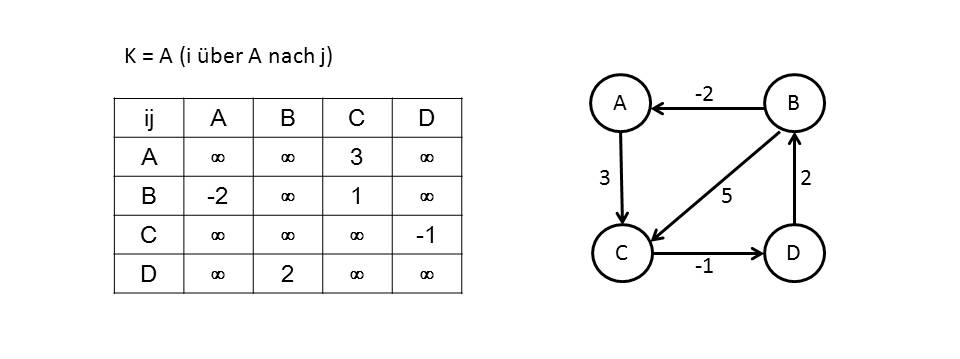
\includegraphics[width=\linewidth]{floyd_warshall_graphs/graph2.JPG}

\end{frame}

%------------------------------------------------

\begin{frame}
\frametitle{Beispiel - Über Knoten B}

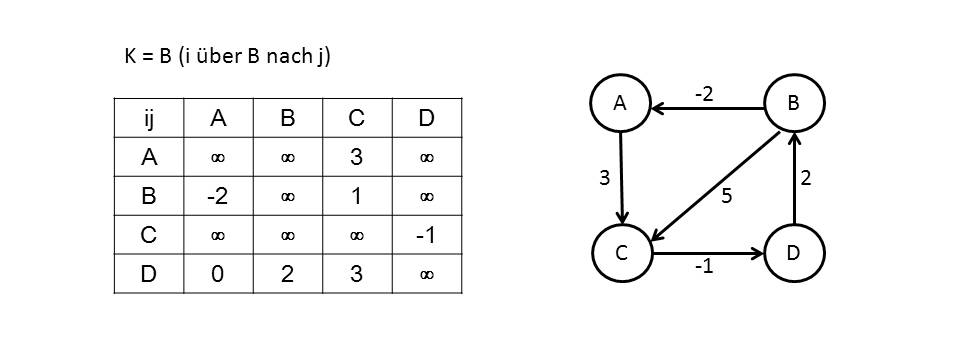
\includegraphics[width=\linewidth]{floyd_warshall_graphs/graph3.JPG}

\end{frame}

%------------------------------------------------

\begin{frame}
\frametitle{Beispiel - Über Knoten C}

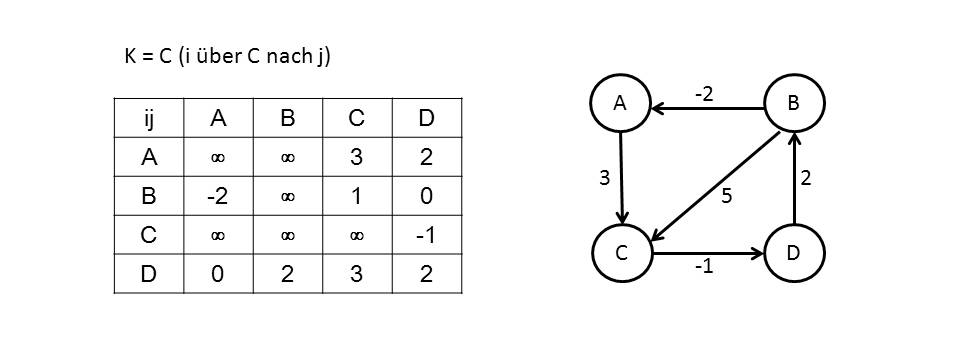
\includegraphics[width=\linewidth]{floyd_warshall_graphs/graph4.JPG}

\end{frame}

%------------------------------------------------

\begin{frame}
\frametitle{Beispiel - Über Knoten D (1)}

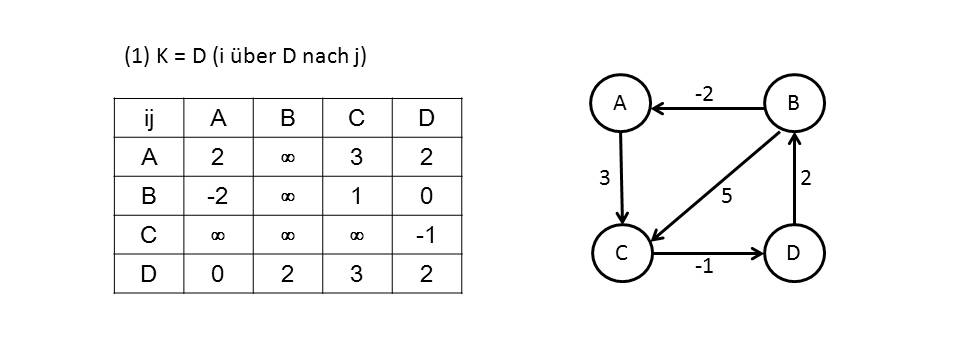
\includegraphics[width=\linewidth]{floyd_warshall_graphs/graph5.JPG}

\end{frame}

%------------------------------------------------

\begin{frame}
\frametitle{Beispiel - Über Knoten D (2)}

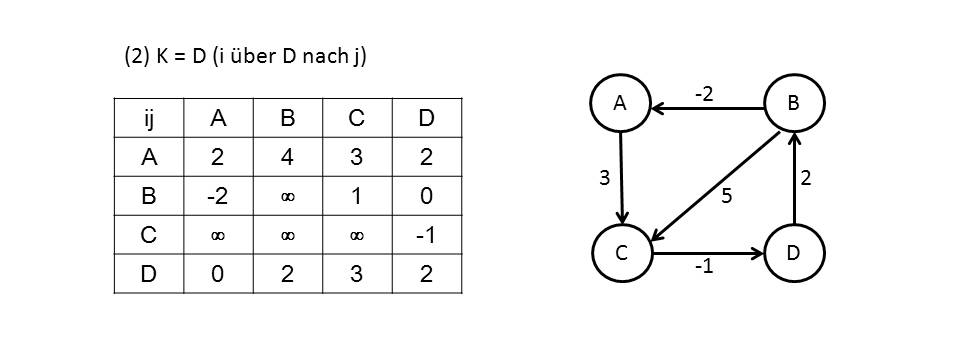
\includegraphics[width=\linewidth]{floyd_warshall_graphs/graph6.JPG}

\end{frame}

%------------------------------------------------

\begin{frame}
\frametitle{Beispiel - Über Knoten D (3)}

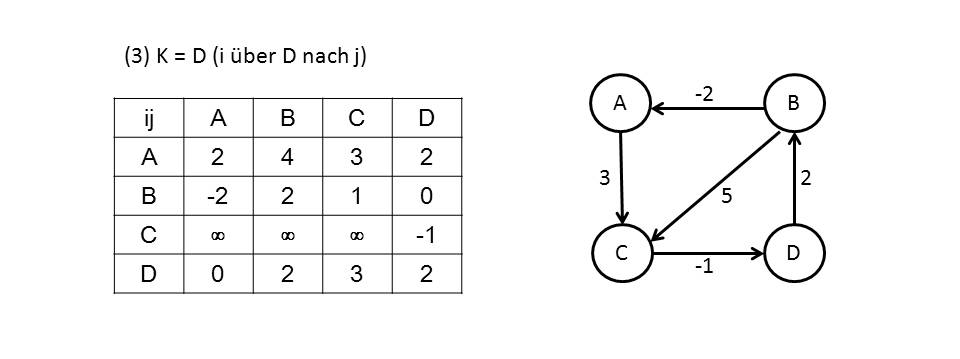
\includegraphics[width=\linewidth]{floyd_warshall_graphs/graph7.JPG}

\end{frame}

%------------------------------------------------

\begin{frame}
\frametitle{Beispiel - Über Knoten D (4)}

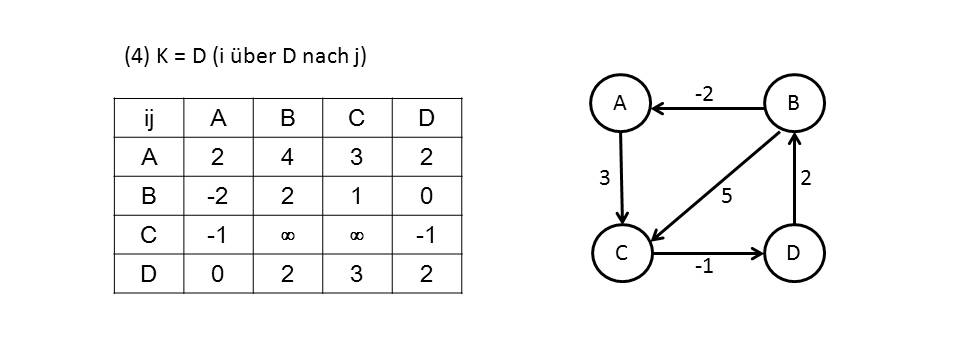
\includegraphics[width=\linewidth]{floyd_warshall_graphs/graph8.JPG}

\end{frame}

%------------------------------------------------

\begin{frame}
\frametitle{Beispiel - Über Knoten D (5)}

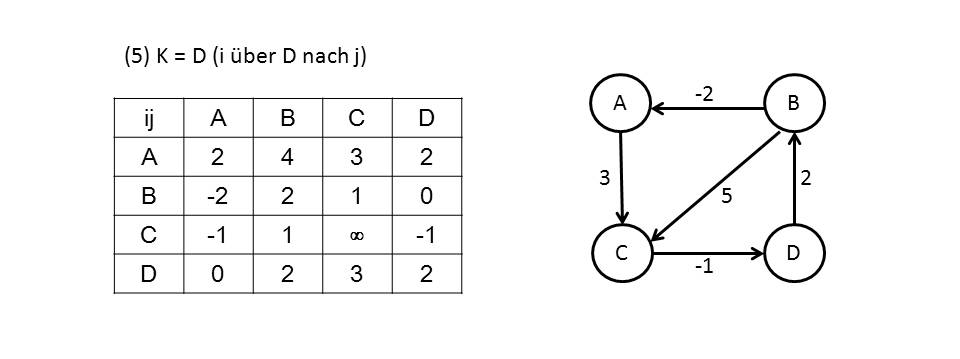
\includegraphics[width=\linewidth]{floyd_warshall_graphs/graph9.JPG}

\end{frame}

%------------------------------------------------

\begin{frame}
\frametitle{Beispiel - Über Knoten D (6)}

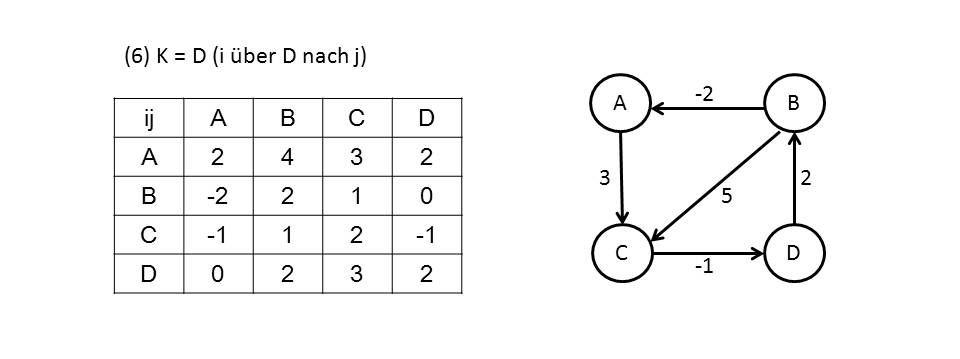
\includegraphics[width=\linewidth]{floyd_warshall_graphs/graph10.JPG}

\end{frame}

%------------------------------------------------

\begin{frame}
\frametitle{Weitere Anwendungen}
\begin{itemize}

\item Auch für SSSP - Probleme anwendbar (wenn $\vert V \vert < 400$)
\item Detektion von negativen oder günstigsten Zyklen möglich $\implies$ ein negativer Zyklus existiert genau dann, wenn ein Diagonaleintrag negativ ist
\item Finden des Durchmessers eines Graphen (der längste der kürzesten Pfade)
\item Minimax, die kleinsten Maximalkosten von allen Wegen
\item Maximin, die größten Minimalkosten von allen Wegen
\end{itemize}
\end{frame}

%------------------------------------------------

\subsection{Beurteilung} 

\begin{frame}
\frametitle{Beurteilung}
\begin{itemize}

\item[+] Asymptotische Komplexität $\in O(n^3)$  und mit Speicher $\in O(n^2)$
\item[+] Sehr leicht zu implementieren (Vierzeiler)
\item[+] Für andere Probleme günstig anzuwenden, wenn $|V|< 400$
\item[-- --] Für andere Probleme \textbf{nur} günstig anzuwenden, wenn $|V|< 400$
\end{itemize}

$\implies$ Gut für das ursprüngliche Problem\\
$\implies$ Auch nützlich für andere Probleme, solange $|V| < 400$
\end{frame}

%------------------------------------------------

\section{Zusammenfassung}

\begin{frame}
\frametitle{Zusammenfassung}
\footnotesize{\begin{table}
\begin{tabular}{l l l l}
\toprule
\textbf{Kriterium} & \textbf{Dijkstra} & \textbf{Bellman Ford} &\textbf{Floyd Warshall}\\
\midrule
Laufzeit & $O((n+m)\log(n))$ & $O(n \cdot m)$ & $O(n^3)$ \\
Max. Größe  & $n,m \leq 300K$ & $n \cdot m \leq 10M$ & $n \leq 400$ \\
Ungewichtet & Ja & Ja (schlecht) & Ja (kleine Graphen) \\
Gewichtet & Ja & Ok & Ja (kleine Graphen) \\
Neg. Kanten & Nein & Ja & Ja \\
Neg. Zyklen & Nein & Ja & Ja \\
Kleine Graphen & Overkill & Overkill & Bestes \\
Kann SSSP? & Ja & Ja & Eingeschränkt \\
\bottomrule
\end{tabular}
\caption{Übersicht}
\end{table}}
Erinnerung: $n:= |V|$ und $m:= |E|$
\end{frame}

%------------------------------------------------